 
%%%%%%%%%%%%%%%%%%%%%%%%%%%%%%%%%%%%%%%%%%%%%%%%%%%%%%%%%%%%%%%%%%%%%
%% This is a (brief) model paper using the achemso class
%% The document class accepts keyval options, which should include
%% the target journal and optionally the manuscript type.
%%%%%%%%%%%%%%%%%%%%%%%%%%%%%%%%%%%%%%%%%%%%%%%%%%%%%%%%%%%%%%%%%%%%%
\documentclass[journal=jpcbfk,manuscript=article]{achemso}

%%%%%%%%%%%%%%%%%%%%%%%%%%%%%%%%%%%%%%%%%%%%%%%%%%%%%%%%%%%%%%%%%%%%%
%% Place any additional packages needed here.  Only include packages
%% which are essential, to avoid problems later. Do NOT use any
%% packages which require e-TeX (for example etoolbox): the e-TeX
%% extensions are not currently available on the ACS conversion
%% servers.
%%%%%%%%%%%%%%%%%%%%%%%%%%%%%%%%%%%%%%%%%%%%%%%%%%%%%%%%%%%%%%%%%%%%%
\usepackage[version=3]{mhchem} % Formula subscripts using \ce{}
\usepackage[T1]{fontenc}       % Use modern font encodings
\usepackage{rotating}


%%%%%%%%%%%%%%%%%%%%%%%%%%%%%%%%%%%%%%%%%%%%%%%%%%%%%%%%%%%%%%%%%%%%%
%% If issues arise when submitting your manuscript, you may want to
%% un-comment the next line.  This provides information on the
%% version of every file you have used.
%%%%%%%%%%%%%%%%%%%%%%%%%%%%%%%%%%%%%%%%%%%%%%%%%%%%%%%%%%%%%%%%%%%%%
%%\listfiles

%%%%%%%%%%%%%%%%%%%%%%%%%%%%%%%%%%%%%%%%%%%%%%%%%%%%%%%%%%%%%%%%%%%%%
%% Place any additional macros here.  Please use \newcommand* where
%% possible, and avoid layout-changing macros (which are not used
%% when typesetting).
%%%%%%%%%%%%%%%%%%%%%%%%%%%%%%%%%%%%%%%%%%%%%%%%%%%%%%%%%%%%%%%%%%%%%
\newcommand*\mycommand[1]{\texttt{\emph{#1}}}

%%%%%%%%%%%%%%%%%%%%%%%%%%%%%%%%%%%%%%%%%%%%%%%%%%%%%%%%%%%%%%%%%%%%%
%% Meta-data block
%% ---------------
%% Each author should be given as a separate \author command.
%%
%% Corresponding authors should have an e-mail given after the author
%% name as an \email command. Phone and fax numbers can be given
%% using \phone and \fax, respectively; this information is optional.
%%
%% The affiliation of authors is given after the authors; each
%% \affiliation command applies to all preceding authors not already
%% assigned an affiliation.
%%
%% The affiliation takes an option argument for the short name.  This
%% will typically be something like "University of Somewhere".
%%
%% The \altaffiliation macro should be used for new address, etc.
%% On the other hand, \alsoaffiliation is used on a per author basis
%% when authors are associated with multiple institutions.
%%%%%%%%%%%%%%%%%%%%%%%%%%%%%%%%%%%%%%%%%%%%%%%%%%%%%%%%%%%%%%%%%%%%%
\author{O. H. Samuli Ollila}
\email{samuli.ollila@helsinki.fi}
%\homepage[]{Your web page}
%\thanks{}
\affiliation{Research Program in Structural Biology and Biophysics, Insititute of Biotechnology, University of Helsinki}
\alsoaffiliation{Institute of Organic Chemistry and Biochemistry,
Czech Academy of Sciences, 
Prague 6, Czech Republic}

\author{Harri A. Heikkinen}
%\homepage[]{Your web page}
%\thanks{}
\affiliation{Research Program in Structural Biology and Biophysics, Insititute of Biotechnology, University of Helsinki}

\author{Hideo Iwa\"i}
%\homepage[]{Your web page}
%\thanks{}
\affiliation{Research Program in Structural Biology and Biophysics, Insititute of Biotechnology, University of Helsinki}


%\author{Andrew N. Other}
%\altaffiliation{A shared footnote}
%\author{Fred T. Secondauthor}
%\altaffiliation{Current address: Some other place, Othert\"own,
%Germany}
%\author{I. Ken Groupleader}
%\altaffiliation{A shared footnote}
%\email{i.k.groupleader@unknown.uu}
%\phone{+123 (0)123 4445556}
%\fax{+123 (0)123 4445557}
%\affiliation[Unknown University]
%{Department of Chemistry, Unknown University, Unknown Town}
%\alsoaffiliation[Second University]
%{Department of Chemistry, Second University, Nearby Town}
%\author{Susanne K. Laborator}
%\email{s.k.laborator@bigpharma.co}
%\affiliation[BigPharma]
%{Lead Discovery, BigPharma, Big Town, USA}
%\author{Kay T. Finally}
%\affiliation[Unknown University]
%{Department of Chemistry, Unknown University, Unknown Town}
%\alsoaffiliation[Second University]
%{Department of Chemistry, Second University, Nearby Town}

%%%%%%%%%%%%%%%%%%%%%%%%%%%%%%%%%%%%%%%%%%%%%%%%%%%%%%%%%%%%%%%%%%%%%
%% The document title should be given as usual. Some journals require
%% a running title from the author: this should be supplied as an
%% optional argument to \title.
%%%%%%%%%%%%%%%%%%%%%%%%%%%%%%%%%%%%%%%%%%%%%%%%%%%%%%%%%%%%%%%%%%%%%
\title[An \textsf{achemso} demo]
      {Rotational Dynamics of Proteins from Spin Relaxation Times and Molecular Dynamics Simulations}

%%%%%%%%%%%%%%%%%%%%%%%%%%%%%%%%%%%%%%%%%%%%%%%%%%%%%%%%%%%%%%%%%%%%%
%% Some journals require a list of abbreviations or keywords to be
%% supplied. These should be set up here, and will be printed after
%% the title and author information, if needed.
%%%%%%%%%%%%%%%%%%%%%%%%%%%%%%%%%%%%%%%%%%%%%%%%%%%%%%%%%%%%%%%%%%%%%
%\abbreviations{IR,NMR,UV}
%\keywords{American Chemical Society, \LaTeX}

%%%%%%%%%%%%%%%%%%%%%%%%%%%%%%%%%%%%%%%%%%%%%%%%%%%%%%%%%%%%%%%%%%%%%
%% The manuscript does not need to include \maketitle, which is
%% executed automatically.
%%%%%%%%%%%%%%%%%%%%%%%%%%%%%%%%%%%%%%%%%%%%%%%%%%%%%%%%%%%%%%%%%%%%%
\begin{document}

%%%%%%%%%%%%%%%%%%%%%%%%%%%%%%%%%%%%%%%%%%%%%%%%%%%%%%%%%%%%%%%%%%%%%
%% The "tocentry" environment can be used to create an entry for the
%% graphical table of contents. It is given here as some journals
%% require that it is printed as part of the abstract page. It will
%% be automatically moved as appropriate.
%%%%%%%%%%%%%%%%%%%%%%%%%%%%%%%%%%%%%%%%%%%%%%%%%%%%%%%%%%%%%%%%%%%%%
\begin{tocentry}
  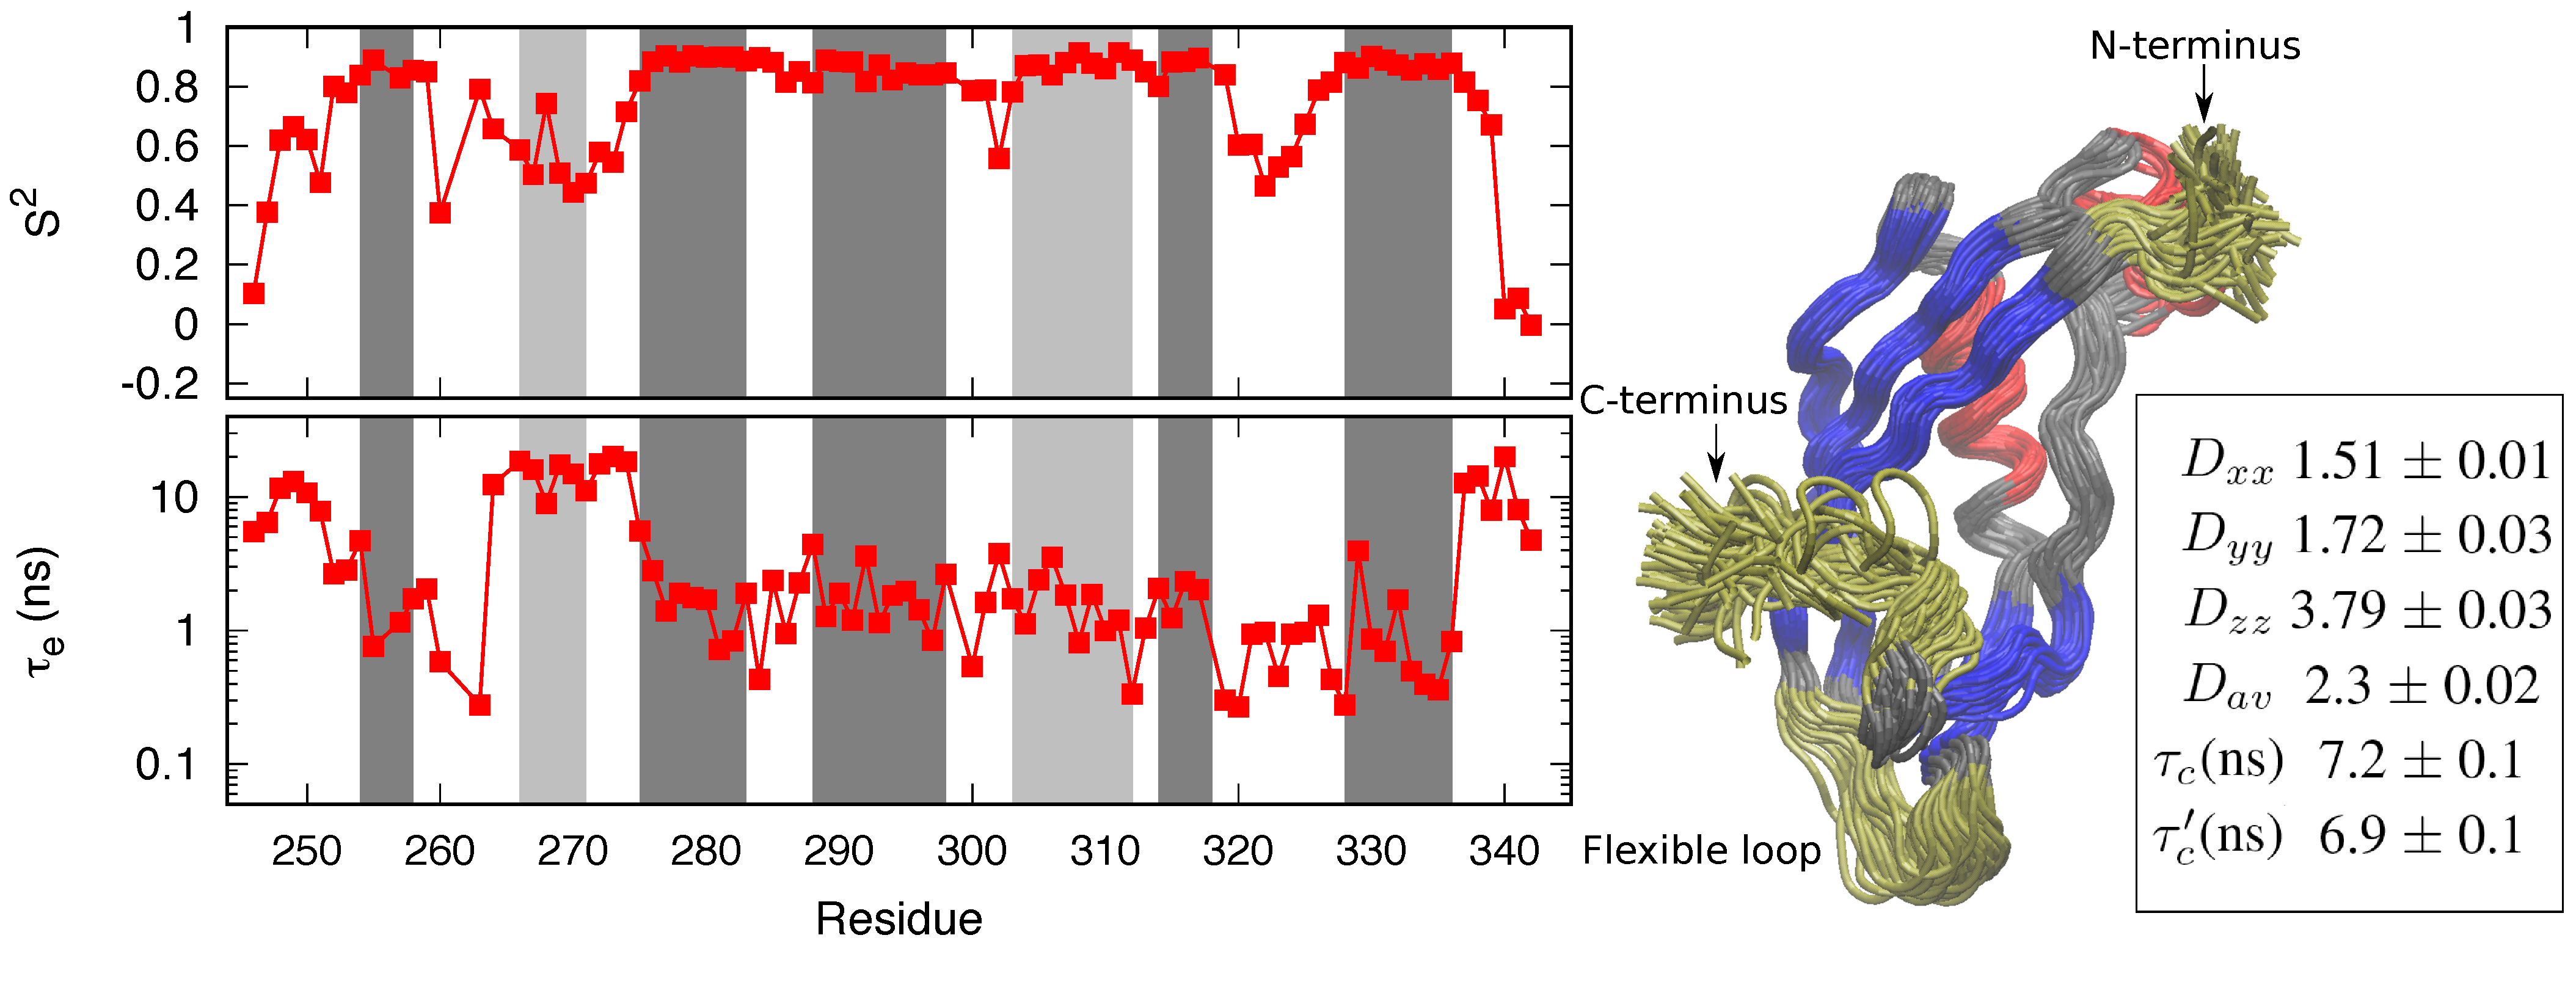
\includegraphics[width=9.0cm]{../Figs/TOC.eps}%
%Some journals require a graphical entry for the Table of Contents.
%This should be laid out ``print ready'' so that the sizing of the
%text is correct.

%Inside the \texttt{tocentry} environment, the font used is Helvetica
%8\,pt, as required by \emph{Journal of the American Chemical
%Society}.

%The surrounding frame is 9\,cm by 3.5\,cm, which is the maximum
%permitted for  \emph{Journal of the American Chemical Society}
%graphical table of content entries. The box will not resize if the
%content is too big: instead it will overflow the edge of the box.

%This box and the associated title will always be printed on a
%separate page at the end of the document.

\end{tocentry}

%%%%%%%%%%%%%%%%%%%%%%%%%%%%%%%%%%%%%%%%%%%%%%%%%%%%%%%%%%%%%%%%%%%%%
%% The abstract environment will automatically gobble the contents
%% if an abstract is not used by the target journal.
%%%%%%%%%%%%%%%%%%%%%%%%%%%%%%%%%%%%%%%%%%%%%%%%%%%%%%%%%%%%%%%%%%%%%
\begin{abstract}
  Conformational fluctuations and rotational tumbling of proteins can be experimentally accessed
  with nuclear spin relaxation experiments. However, interpretation of molecular dynamics from the
  experimental data is often complicated, especially for molecules with anisotropic
  shape. Here we apply classical molecular dynamics simulations to interpret the conformational fluctuations
  and rotational tumbling of proteins with arbitrarily anisotropic shape. The direct calculation
  of spin relaxation times from simulation data did not reproduce the experimental data.
  This was successfully corrected by scaling the overall rotational diffusion coefficients around the
  protein inertia axes with a constant factor. The achieved good agreement with experiments
  allowed the interpretation of the internal and overall dynamics of proteins with significantly
  anisotropic shape. The overall rotational diffusion was found to be Brownian, having only a
  short subdiffusive region below 0.12~ns. The presented methodology can be applied to
  interpret rotational dynamics and conformation fluctuations of proteins with arbitrary anisotropic
  shape. However, a water model with more realistic dynamical properties is probably required
  for intrinsically disordered proteins.
\end{abstract}

%%%%%%%%%%%%%%%%%%%%%%%%%%%%%%%%%%%%%%%%%%%%%%%%%%%%%%%%%%%%%%%%%%%%%
%% Start the main part of the manuscript here.
%%%%%%%%%%%%%%%%%%%%%%%%%%%%%%%%%%%%%%%%%%%%%%%%%%%%%%%%%%%%%%%%%%%%%
\section{Introduction}

Conformational fluctuations and the entropy of proteins
play a significant role in their functionality
and interactions with other biomolecules.
Conformational fluctuations and the overall Brownian tumbling of proteins
are experimentally accessible through the 
spin relaxation times of $^{15}$N and $^{13}$C nuclei measured
with nuclear magnetic resonance (NMR) 
techniques \cite{jarymowycz06,korzhnev01,mulder01,eisenmesser05,bedem15,lewandowski15,lamley15}. 
The spin relaxation rates have been used to, for example, analyze
conformational entropies \cite{yang96,kasinath13,allner15,jarymowycz06,solomentsev18}, binding entropies \cite{akke93,jarymowycz06},
resolve sampled structures \cite{mulder01,eisenmesser05,bedem15,medina14}
and validate molecular dynamics simulations \cite{best04,showalter07a,showalter07b,maragakis08,trbovic08,debiec16,hoffmann18,debiec18}.
These analyzes are almost exclusively based on the
separation of the internal conformational fluctuations 
and the overall rotational tumbling \cite{wennerstrom79,Lipari82}.
Also the isotropic overall diffusion is often assumed, while
analysis of anisotropic molecules is significantly more
complicated \cite{woessner62,shimizu62,jarymowycz06,korzhnev01,luginbuhl97,hall04}.
Thus, the new approaches are needed to interpret spin relaxation times
measured from anisotropic or intrinsically disordered molecules.

Classical molecular dynamics (MD) simulation methods are
promising tools to interpret spin relaxation experiments
for molecules with significantly anisotropic shape or correlations between
internal and overall rotational motions. Practical applications
are, however, limited by inaccuracies in the force field descriptions
and the available time scales in the simulations \cite{prompers02,maragakis08,trbovic08,wong08,anderson12,salvi16,debiec16}.
The main issues have been the overestimated overall rotational diffusion of proteins
due to inaccuracies in water models~\cite{wong08,takemura12,debiec16} and the
insufficient accuracy of correlation functions calculated from
single molecules in MD simulations~\cite{lu06,anderson12}.

In this work we overcome these issues by assuming that the overall
rotational dynamics of protein follows anisotropic rigid body diffusion.
Diffusion coefficients around inertia axes are 
directly calculated from angular displacements.
The diffusion coefficients are then used to determine the
contribution of the overall rotational tumbling to the 
rotational correlation functions of N-H bonds.
This reduces the required simulation length for the accurate determination
of the rotational correlation functions. Furthermore, the overestimated
overall Brownian tumbling rates due to the inaccurate water model
can be corrected during the correlation function calculation by scaling
the diffusion coefficients in all directions with a constant factor.
The corrected correlation functions can be used to interpret the spin relaxation
experiments for proteins with arbitrarily anisotropic shapes.

The developed approach is demonstrated by interpreting the experimental spin relaxation data 
of C-terminal domains of TonB proteins from {\it Helicobacter pyroli} ({\it Hp}TonB-92)~\cite{ciragan16}
and from {\it Pseudomonas aeruginosa} ({\it Pa}TonB-96)~\cite{oeemig17}, having
92 and 96 residues, respectively. Both proteins have significantly
anisotropic shape, which would complicate the standard spin relaxation data
analysis~\cite{woessner62,shimizu62,jarymowycz06,korzhnev01,luginbuhl97,hall04}.


\section{Methods}

\subsection{Spin relaxation experiments and rotational dynamics of molecules}
Molecular dynamics of the protein backbone residues and spin relaxation experiments can
be connected by using the spectral density $J(\omega)$ 
\begin{equation}\label{SPECTdens}
  J(\omega)=2\int_0^\infty C(t) \cos(\omega t) {\rm d}t,
\end{equation}
which is the Fourier transformation of the second order
rotational correlation function for N-H bond vector
\begin{equation}\label{CORRFdef}
  C(t)=\langle \frac{3}{2}\cos^2\theta_{t'+t}-\frac{1}{2} \rangle_{t'},
\end{equation}
where $\theta_{t'+t}$ is the N-H bond angle between times $t'$ and $t'+t$
and angular brackets refer to the ensemble average.
Connection to the experimentally measured spin relaxation times $T_1$, $T_2$
and the NOE relaxation are given by the Redfield equations~\cite{abragam,kay89}
\begin{equation}\label{R1}
  \begin{aligned}
  \frac{1}{T_1}= & \frac{d_{\rm{NH}}^2N_{\rm{H}}}{20}\bigg[J(\omega_{\rm{H}}-\omega_{\rm{N}})+3J(\omega_{\rm{N}})+6J(\omega_{\rm{N}}+\omega_{\rm{H}})\bigg] \\
        & +\frac{(\sigma \omega_{\rm{N}})^2}{15}J(\omega_{\rm{N}}),
  \end{aligned}
\end{equation}
\begin{equation}\label{R2}
    \begin{aligned}
  \frac{1}{T_2}= & \frac{1}{2}\frac{d_{\rm{NH}}^2N_{\rm{H}}}{20}\bigg[4J(0)+3J(\omega_{\rm{N}})+J(\omega_{\rm{H}}-\omega_{\rm{N}})+6J(\omega_{\rm{H}})  \\
    & +6J(\omega_{\rm{N}}+\omega_{\rm{H}})\bigg]+\frac{(\sigma \omega_{\rm{N}})^2}{90}[4J(0) +3J(\omega_{\rm{N}})],
    \end{aligned}
\end{equation}
\begin{equation}\label{NOE}
  {\rm NOE}=1+\frac{d_{\rm{NH}}^2N_{\rm{H}}}{20}\bigg[6J(\omega_{\rm{N}}+\omega_{\rm{H}})+J(\omega_{\rm{H}}-\omega_{\rm{N}}))\bigg]\frac{\gamma_{\rm{H}}T_1}{\gamma_{\rm{N}}},
\end{equation}
where $\omega_{\rm{N}}$ and $\omega_{\rm{H}}$ are the Larmor angular
frequencies of $^{15}$N and $^1$H respectively, and
the number of bound protons $N_{\rm{H}}=1$ for N-H bonds.
The dipolar coupling constant is given by
\begin{equation}
d_{\rm{NH}}=-\frac{\mu_0\hbar\gamma_{\rm{H}}\gamma_{\rm{N}}}{4\pi\langle r_{\rm{NH}}^3\rangle},\nonumber
\end{equation}
where $\mu_0$ is the magnetic constant or vacuum permeability, $\hbar$ is the reduced Planck constant,
$\gamma_{\rm{N}}$ and $\gamma_{\rm{H}}$ are the gyromagnetic constants of $^{15}$N and $^1$H, respectively.
The average cubic length is calculated as $\langle r_{\rm{NH}}^3\rangle = (0.101$ ${\rm nm})^3$ and the 
value of $\Delta \sigma = -160$ ppm is used for the chemical shift anisotropy of N-H bonds in 
proteins \cite{kay89,hiyama88}.

Spin relaxation experiments are typically interpreted for proteins by
assuming that the motions related to the overall Brownian tumbling 
and conformational fluctuations are independent \cite{halle09}.
The rotational correlation function for each N-H bond can be then written
as  \cite{wennerstrom79,Lipari82,jarymowycz06,korzhnev01,halle09}
\begin{equation}\label{CORRFsep}
  C(t)=C_I(t)C_O(t),
\end{equation}
where $C_I(t)$ and $C_O(t)$ are correlation functions for the internal dynamics and overall
rotations, respectively. Conformational fluctuations can be described
in this approximation by using the square of the order parameter respect to 
molecular axes $S^2$, which is given by the plateau of the internal rotational 
correlation function. Timescales for the fluctuations can be characterized by
using the effective correlation time 
\begin{equation}\label{effCT}
  \tau_{\rm eff}=\int_0^\infty C_I'(t) \mathrm{d}t,
\end{equation}
where $C_I'(t)=\frac{C_I-S^2}{1-S^2}$ is the reduced correlation function \cite{Lipari82}.

The overall rotational correlation function is often described
by approximating the protein as a rigid body.
For arbitrarily anisotropic molecules, the correlation functions
can  be presented as a sum of five exponentials~\cite{woessner62,korzhnev01}
\begin{equation}\label{CORRFanisot}
  C_O(t)=\sum_{j=1}^5 A_j e^{-t/\tau_j},
\end{equation}
where the prefactors $A_j$ depend on the directions of chemical bonds 
respect to the molecular axes \cite{woessner62,luginbuhl97} and
the time constants $\tau_j$ are related 
to the diffusion constants around
three principal axes of a molecule
($D_{x}$, $D_{y}$, and $D_{z}$) through equations~\cite{woessner62,korzhnev01}
\begin{equation}\label{tauDIFFeq}
  \begin{split}
  \tau_1&=(4D_{x}+D_{y}+D_{z})^{-1} \\
  \tau_2&=(D_{x}+4D_{y}+D_{z})^{-1} \\
  \tau_3&=(D_{x}+D_{y}+4D_{z})^{-1} \\
  \tau_4&=[6(D_{\rm av}+(D_{\rm av}^2-L^2)^{-1/2}]^{-1} \\
  \tau_5&=[6(D_{\rm av}-(D_{\rm av}^2-L^2)^{-1/2}]^{-1}, \\
  \end{split}
\end{equation}
where $D_{\rm av}=\frac{1}{3}(D_{x}+D_{y}+D_{z})$ and 
$L^2=\frac{1}{3}(D_{x}D_{y}+D_{x}D_{z}+D_{y}D_{z})$.

The simplest approach to extract molecular dynamics from the experimental
data is the original ''model-free analysis''~\cite{Lipari82},
where an isotropic diffusion is assumed for the overall rotation of the protein.
This reduces Eq.~\ref{CORRFanisot} to a monoexponential form and the overall rotational
dynamics can be described with a single time constant $\tau_c$.
Also the internal correlation functions for each residue are assumed
to decay exponentially with a single time constant $\tau_{\rm eff}$
toward to the square of the order parameter $S^2$. The three parameters
($\tau_c$, $\tau_{\rm eff}$, and $S^2$) can be then successfully resolved from a
fit to the experimental data.
However, the number of parameters to be fitted increases if the protein
experiences an anisotropic overall diffusion or has several timescales for internal motions.
In this case the fitting becomes often ambiguous, even if the experimental data
would be measured with multiple magnetic field strengths~\cite{dosset00,luginbuhl97,jarymowycz06}.
The anisotropic rotational diffusion is sometimes described with hydrodynamical
calculations, but they are sensitive to the estimation of the
hydration shell around the protein~\cite{torre00}.

Rough estimate for the timescale of overall rotational dynamics 
is often given by using the $T_1/T_2$ ratio \cite{kay89}. 
This is based on the assumptions that $T_1$ and $T_2$
are independent of the internal motions and that the overall
dynamics is isotropic. The spectral density then reduces to 
\begin{equation}
J'(\omega) = S^2\frac{\tau_c'}{1+(\omega \tau_c')^2} 
\end{equation}
and the correlation time describing the overall rotational motion, $\tau_c'$, can 
be estimated by numerically minimizing the equation
%\begin{widetext}
\begin{equation}\label{ratioEQ}
  \frac{T_1}{T_2} \approx  \frac{\frac{1}{2}\frac{d_{\rm{NH}}^2N_{\rm{H}}}{20}\bigg[4J'(0)+3J'(\omega_{\rm{N}})+J'(\omega_{\rm{H}}-\omega_{\rm{N}})+6J'(\omega_{\rm{H}})  +6J'(\omega_{\rm{N}}+\omega_{\rm{H}})\bigg]+\frac{(\sigma \omega_{\rm{N}})^2}{90}[4J'(0) +3J'(\omega_{\rm{N}})]}{\frac{d_{\rm{NH}}^2N_{\rm{H}}}{20}\bigg[J'(\omega_{\rm{H}}-\omega_{\rm{N}})+3J'(\omega_{\rm{N}})+6J'(\omega_{\rm{N}}+\omega_{\rm{H}})\bigg] +\frac{(\sigma \omega_{\rm{N}})^2}{15}J'(\omega_{\rm{N}})}
\end{equation}
%\end{widetext}
with respect to the experimentally measured $T_1/T_2$ ratio.

\subsection{Rotational dynamics from molecular dynamics simulations}\label{MDanalysis}
A classical molecular dynamics simulation gives a trajectory for each atom in
the system as a function of time. Rotational correlation functions for each bond
can be then directly calculated from the trajectories by Eq. \ref{CORRFdef}
and used to calculate the spin relaxation times through Eqs. \ref{SPECTdens}-\ref{NOE}.
The resulting values can be compared to experimental data in order to assess simulation model
quality \cite{best04,showalter07a,showalter07b,maragakis08,trbovic08,fisette12,debiec18,debiec16,salvi16,hoffmann18} and
to interpret experiments~\cite{fisette12,debiec18,anderson17}.

The direct comparison with experiments is, however, often complicated by
the insufficient statistics for the calculated correlation functions and the overestimated
rotational diffusion due to inaccuracies in the used water models~\cite{wong08,anderson12,takemura12}.
Here we show that the statistical accuracy of the contribution of the
overall tumbling to the correlation functions, $C_0(t)$ in Eq.~\ref{CORRFsep}, can be increased for
rigid proteins by directly calculating the diffusion coefficients of the inertia axes.
The rotational diffusion coefficients can be related to the timescales $\tau_j$
of the correlation function for anisotropic rigid body rotation
in Eq.~\ref{CORRFanisot} by using the relations in Eq.~\ref{tauDIFFeq}~\cite{woessner62}.

The rotational diffusion coefficients are calculated by fitting a linear slope to the 
square angle deviation of the inertia axes (see below).
Lag times up to one hundredth of the total simulation length were used.
This is expected to be the maximum lag time for the good statistics
of rotational dynamics analyzed from a single molecule in MD simulations~\cite{lu06}.
Error bars for the diffusion coefficients were defined to include results when the lag
time was varied with $\pm$1 ns.
This requires less simulation data
for the good statistics than a direct fit of the multiexponential sum in Eq. \ref{CORRFanisot}
to the rotational correlation function calculated from MD simulation.
In addition, the overestimated rotational diffusion due to water model~\cite{wong08,takemura12,debiec16} can
be corrected by scaling the diffusion coefficients around all inertia axes
by a constant factor. This approach takes into account the anisotropic shape of
the molecule. This is a significant advancement to the previous studies, which assume
isotropic rotational diffusion with a single exponential rotational correlation
function \cite{showalter07a,showalter07b,maragakis08,gu14,allner15} or
use order parameters to compare simulations with experimental data~\cite{gu14,maragakis08,trbovic08,best04}.


The practical analysis can be divided into seven steps: \\
1) The total rotational correlation functions $C(t)$
for N-H bond vectors in a protein are directly calculated from MD simulation trajectory
by applying Eq.~\ref{CORRFdef}. \\
2) The rotational correlation functions for internal
dynamics $C_I(t)$ are calculated from MD simulation trajectory
by removing overall rotation of the protein. \\
3) The overall and internal motions are assumed to be independent and the overall
rotational correlation function is calculated from Eq. \ref{CORRFsep} as $C_O(t)=C(t)/C_I(t)$. \\
4) The mean square angle deviations of rotation around protein inertia axes
are calculated from MD simulation trajectory. \\
5) Rotational diffusion constants $D_x$, $D_y$, and $D_z$ around inertia axes
are calculated by fitting a straight line to the mean square angle deviations 
\begin{equation}\label{DIFFdef}
  \begin{aligned}
    \langle \Delta \alpha_{t'+t}^2 \rangle_{t'} = 2 D_{x} t \\
    \langle \Delta \beta_{t'+t}^2 \rangle_{t'} = 2 D_{y} t \\
    \langle \Delta \gamma_{t'+t}^2 \rangle_{t'} = 2 D_{z} t, \\
  \end{aligned}
\end{equation}
where $\langle \Delta \alpha_{t'+t}^2 \rangle_{t'}$,
$\langle \Delta \beta_{t'+t}^2 \rangle_{t'}$, and
$\langle \Delta \gamma_{t'+t}^2 \rangle_{t'}$ are
the mean square angle deviations from the shortest protein
inertia axis to the longest, respectively.\\
6) Contribution of the overall rotational tumbling to all correlation
functions is assumed to follow Eq.~\ref{CORRFanisot} with the
timescales $\tau_j$ calculated from the rotational diffusion constants
by using the relations in Eq.~\ref{tauDIFFeq}.
Weighting factors $A_j$ are determined by fitting the equation %with new timescales
to the overall rotational correlation functions calculated from MD simulations in step 3. \\
7) The new correlation functions are calculated by substituting
internal correlation functions, $C_I(t)$, from step 2 and anisotropic rigid body
rotational correlation functions, $C_O(t)$, from step 6 to
Eq.~\ref{CORRFsep} giving
\begin{equation}\label{newCORRF}
  C_N(t)=C_I(t)\sum_{j=1}^5 A_j e^{-t/\tau_j}.
\end{equation}
These correlation functions are then used to calculate spin relaxation times
from Eqs. \ref{SPECTdens}-\ref{NOE}. The incorrect overall rotational
diffusion due to a water model can be corrected at this point  by scaling the rotational diffusion
coefficients, i.e. timescales $\tau_j$, with a constant factor before calculating
new correlation functions from Eq. \ref{newCORRF}.
Here we determine the optimal scaling factors separately for each system.
Scaling factors between 1--4 are explored with the spacing of 0.1 and
the value giving the best agreement with the experimental spin relaxation data
is the optimal scaling factor.


\subsection{Simulation and analysis details}
\begin{sidewaystable}[hp]
\centering
\caption{Simulated systems and rotational diffusion coefficients (rad$^2\cdot 10^7$/s) calculated from simulations.
}\label{ROTdiffCOEFFS}
\begin{tabular}{c c c c c c c c c c c c c c c c}
Protein     & Water\footnote{Water model used in simulation.} & T (K)\footnote{Simulation temperature}  &  $t_{\rm s}$(ns)\footnote{Total simulation time}  &  $t_{\rm a}$(ns)\footnote{Analyzed simulation time}  & $D_{x}$ &&$D_{y}$ &&$D_{z}$ &&$D_{||}/D_\perp$\footnote{$D_{||}=D_{z}$, $D_\perp=\frac{1}{2}(D_{x}+D_{y})$} & &$D_{\rm av}$\footnote{$D_{\rm av}=\frac{1}{3}(D_{x}+D_{y}+D_{z} )$}& &files \\
\hline
{\it Pa}TonB-96      & tip3p       & 298    & 400                 &  300                 & 4.2 $\pm$ 0.1 && 4.4 $\pm$ 0.1 && 10.4 $\pm$ 0.1 && 2.42 $\pm$ 0.1 && 6.4 $\pm$ 0.1 && [\citenum{PsTonB-tip3p-298K}] \\
{\it Pa}TonB-96      & tip4p       & 298    & 400                 &  390                 & 1.81 $\pm$ 0.01 && 2.06 $\pm$ 0.03 && 4.55 $\pm$ 0.03 && 2.35 $\pm$ 0.04 && 2.80 $\pm$ 0.02 && [\citenum{PsTonB-tip4p-298K}] \\
{\it Pa}TonB-96      & tip4p       & 310    & 400                 &  390                 &  2.60 $\pm$ 0.02 &&  2.22 $\pm$ 0.05& &  5.0  $\pm$ 0.1  & &  2.07 $\pm$ 0.09& &   3.26 $\pm$  0.07 && [\citenum{PsTonB-tip4p-310K}]\\
{\it Pa}TonB-96      & OPC4        & 310    & 1200                &  1190                &  2.01 $\pm$ 0.01 && 2.19 $\pm$ 0.01 && 5.01 $\pm$  0.03 && 2.39 $\pm$ 0.02 && 3.07 $\pm$ 0.01 && [\citenum{PsTonB-OPC4-310K}]  \\
\hline
{\it Hp}TonB-92      & tip3p       & 310    & 570                   &  370                 & 8.25 $\pm$ 0.05 && 7.67 $\pm$ 0.06 && 15.9 $\pm$ 0.3 && 1.99 $\pm$ 0.06 &&  10.6 $\pm$ 0.2 &&  [\citenum{HpTonB-tip3p-310K}] \\
{\it Hp}TonB-92      & tip3p       & 303    & 800                   &  790                 & 6.24 $\pm$ 0.02 && 7.04 $\pm$ 0.03 && 11.9 $\pm$ 0.2 && 1.80 $\pm$ 0.03 && 8.40 $\pm$ 0.07 && [\citenum{HpTonB-tip3p-303K}] \\
{\it Hp}TonB-92      & tip4p       & 310    & 470                   &  370                 & 3.6 $\pm$ 0.1 && 3.24 $\pm$ 0.01 && 6.3 $\pm$ 0.3 && 1.8 $\pm$ 0.1 && 4.4 $\pm$ 0.2 && [\citenum{HpTonB-tip4p-310K}] \\
{\it Hp}TonB-92      & tip4p       & 303    & 400                   &  200                 & 2.7 $\pm$ 0.1 && 2.71 $\pm$ 0.02 && 5.6 $\pm$ 0.5 && 2.1 $\pm$ 0.2 && 3.7 $\pm$ 0.2 && [\citenum{HpTonB-tip4p-303K}] \\
{\it Hp}TonB-92      & OPC4        & 310    & 800                   &  790                 & 2.85 $\pm$ 0.01 && 2.70 $\pm$ 0.01 && 5.56 $\pm$ 0.01 && 2.00 $\pm$ 0.01 && 3.70 $\pm$ 0.01 && [\citenum{HpTonB-OPC4-310K}] \\
\end{tabular}
\end{sidewaystable}
All simulations were performed using Gromacs 5 \cite{abraham15}
and Amber ff99SB- ILDN~\cite{lindorff10} force field for proteins. The protein was solvated
to tip3p\cite{jorgensen83}, tip4p \cite{jorgensen83}, or OPC4 \cite{izadi14} water models.
Initial structures were taken from the lowest energy NMR structures of {\it Hp}TonB-92 (PDB code: 5LW8) \cite{ciragan16} and
{\it Pa}TonB-96 (PDB code: 6FIP) \cite{oeemig17}.
The temperature was coupled to the desired value with the v-rescale thermostat \cite{bussi07} and the pressure was 
isotropically set to 1 bar using Parrinello-Rahman barostat \cite{parrinello81}.
Timestep was 2~fs, Lennard-Jones interactions were cut-off at 1.0~nm,
PME~\cite{darden93,essman95} was used for electrostatics and LINCS was used
to constrain all bond lengths \cite{hess07}. The simulated systems are listed
in Table \ref{ROTdiffCOEFFS} with the references giving access to the trajectories
and the related simulation files. Equilibration of the trajectories were followed
by monitoring the protein RMSD, intertia tensor eigenvalues and rotation angles.
Sufficient amount of trajectory was omitted to remove the significant fluctuations in
these parameters in the beginning of simulation. If such fluctuations were
not observed, the first 10ns of the trajectory was omitted as an equilibration period.

The rotational correlation functions are calculated with {\it gmx rotacf} from
Gromacs package \cite{gromacsMANUAL}. The overall rotation was removed
for $C_I(t)$ calculation by using a fit option of the {\it gmx trjconv} tool
in Gromacs package \cite{gromacsMANUAL}. The order parameters $S^2$
were determined by averaging rotational correlation functions from
oriented trajectory, $C_I(t)$, over the lag times above 50~ns.
The effective correlation times were then calculated by Eq.~\ref{effCT}. 
Inertia axes of proteins were calculated with {\it compute\_inertia\_tensor}
function from MDTraj python library~\cite{McGibbon2015MDTraj}.

Spectral density was calculated by fitting a
sum of 471 exponentials with timescales from 1 ps to 50 ns
with logarithmic spacing
\begin{equation}\label{gprime_fit}
C_N(t)=\sum_{i=1}^{N}\alpha_i e^{-t/\tau_i}
\end{equation}
to the new correlation function from Eq.~\ref{newCORRF}
by using the {\it lsqnonneg} routine in MATLAB \cite{matlab}.
The Fourier transform was then calculated by using the analytical function
for the sum of exponentials 
\begin{equation}\label{FTanal}
J(\omega) =  2 \sum_{i=1}^{N}\alpha_i\frac{\tau_i}{1+\omega^2\tau_i^2}.
\end{equation}
A similar approach has been previously used for the lamellar lipid and surfactant
systems in combination with solid state NMR experiments \cite{nowacka13,ferreira15}.
All the computer programs used for the analysis are available at~\cite{proteindynamicsGIT}.

\subsection{Spin relaxation experiments}
NMR experiments were recorded on a Bruker Avance III 850 NMR spectrometer equipped
with cryogenic probe head. The longitudinal ($T_1$), transverse ($T_2$), and
$^1$H-$^{15}$N-heteronuclear NOE spin relaxation times
for the backbone $^{15}$N atoms of {\it Hp}TonB-92~\cite{ciragan16}
were collected at 303~K using the well-established NMR pulse sequences described previously~\cite{kay89,barbato92}.
The similarly detected spin relaxation data for {\it Pa}TonB-96 at 298~K is also reported in a another publication~\cite{oeemig17}. 
The $T_1$ and $T_2$ relaxation times were measured using the following delay
times: 10, 50, 100, 200, 300, 500, 800, 1000, 1200 and 2000 ms,
and 16, 64, 96, 128, 156, 196, 224 and 256 ms for CPMG pulse train with 1.0 ms interval
for $T_2$ relaxation times, respectively. The relaxation rates ($R_1=1/T_1$, $R_2=1/T_2$)
were calculated as an exponential fit of a single exponential decay to peak intensity
values: $I(t) = I_0 \exp(-t/T_1)$, or $I(t)=I_0 \exp(-t/T_2)$,
where $I(t)$ is the peak volume at a time $t$. The $^{15}$N$ \{ ^1$H$ \} $-NOE measurements were carried out
with a relaxation delay of 5~s with and without saturation of the amide protons.
The $^{15}$N$ \{ ^1$H$ \} $-NOE values were derived from the volumes of the HSQC peaks using the
equation of $\nu=I/I_0$. The relaxation data was processed and analyzed using
Bruker Dynamic Center software (version 2.1.8).

\section{Results and Discussion}

\subsection{Global rotational dynamics of protein}

The mean square angle deviations for the rotation of {\it Pa}TonB-96 protein construct
around inertia axes in the simulation with OPC4 water model
are shown in Fig. \ref{RMASDplot}. This is the longest
simulation data set in this work (1.2 $\mu$s) and the
linear behavior of the mean square angle deviations are observed
for the lag times up to one hundredth of the total simulation length (12~ns),
which is expected to be the maximum lag time for the good statistics
of rotational dynamics analyzed from a single molecule in MD simulations~\cite{lu06}.
Deviations from the linear behavior are only seen with the lag times longer
than this limit, as also demonstrated for the shorter simulations
with tip4p water at two different temperatures
in Figs.~S1~and~S2 in Supplementary Information.
The plots with log-log scale in
Figs.~\ref{RMASDplot},~S1~and~S2
reveal a weakly subdiffusive region only below very short timescales
of approximately~0.12~ns. Thus, we conclude that the protein
experiences the Brownian rotational tumbling with  a good approximation.
The diffusion coefficients can be then calculated from the slope of the mean square angle
deviations according to Eq. \ref{DIFFdef} by using the lag times less than
one hundredth of the total MD simulation length.
The error bars were calculated varying the lag time with 1~ns to both directions.
The data from {\it Hp}TonB-92 protein (not shown) led to similar conclusions.
\begin{figure}[htb]
  \includegraphics[width=8.0cm]{../Figs/RMASDplotPsTonBOPC4.eps}%
  \caption{Mean square angle deviations of inertia tensor axes calculated from
    {\it Pa}TonB-96 simulation with OPC water model. The data shown with linear (top) and logarithmic scale (bottom).
    \label{RMASDplot}}%
\end{figure}

The resulting rotational diffusion constants from different simulations are
summarized in Table \ref{ROTdiffCOEFFS}.
As expected, the rotational diffusion coefficients
increase with the temperature and the decreasing size of a protein.
The values are, however, larger than 
expected from the experimental $T_1/T_2$ ratio analyzed with Eq. \ref{ratioEQ}
and from the previously reported values for proteins with similar
sizes~\cite{krishnan98}, especially when tip3p water model is used.
Similar results were previously explained by the overestimated water
self-diffusion of tip3p water model~\cite{wong08,takemura12,debiec16}.

The analysis leading to the new correlation functions in Eq.~\ref{newCORRF}
(see Methods section) is exemplified in
Fig.~\ref{exampleCORRF} for three residues locating in different domains of {\it Pa}TonB-96
with different characteristic rotational dynamics.
The flexible C-terminus is represented by the residue 341,
more rigid $\beta$-sheet by the residue 331 and a
flexible loop between two $\beta$-strands by residue 322
(see the labeling in Fig. \ref{PsTonBrelaxationDATAscaled}). 
The total correlation functions $C(t)$
of all the residues in Fig.~\ref{exampleCORRF}  (top, solid lines) 
decay toward zero within~$\sim$10-50~ns.
The internal correlation functions $C_I(t)$ in Fig.~\ref{exampleCORRF} (middle)
decay to a plateau value, which defines the square of the order parameter $S^2$.
As expected, the internal correlation function for residue 331 in the
rigid $\beta$-sheet rapidly decays to the largest order parameter value,
while the correlation functions of the residues in the loop and C-terminus 
decay slower to the smaller order parameter values due to the larger conformational ensemble
sampled by these regions.

\begin{figure}[!h]
  \includegraphics[width=8.5cm]{../Figs/exampleCORRF2.eps}%
  \caption{Rotational correlation functions calculated from MD simulations of {\it Pa}TonB-96 with tip4p water
    model at 298~K for residues at different regions.
    (top) total correlation functions $C(t)$ calculated from MD simulation (solid lines) and
    new correlation functions determined from Eqs. \ref{CORRFsep} and \ref{CORRFanisot} by
    using rotational diffusion constants and fitted prefactors (dashed lines),
    (middle) correlation functions for internal motions calculated from simulation with removed overall protein rotation
    (bottom) correlation function for overall motions determined as $C_O(t)=C(t)/C_I(t)$ (solid lines) and by fitting
    to Eq. \ref{CORRFanisot} with timescales from rotational diffusion coefficients in Table~\ref{ROTdiffCOEFFS} (dashed lines).
    }\label{exampleCORRF}
\end{figure}

The overall rotational correlation functions, $C_O(t)=C(t)/C_I(t)$,
are shown in Fig.~\ref{exampleCORRF} (bottom, solid lines).
Also the correlation functions of anisotropic rigid body rotation
from Eq. \ref{CORRFanisot} are shown in Fig. \ref{exampleCORRF} (bottom, dashed lines).
The timescales for the latter, $\tau_i$, are given by the rotational
diffusion coefficients from the simulation and the relations
in Eq.~\ref{tauDIFFeq}. The prefactors, $A_j$, are determined by fitting
Eq.~\ref{CORRFanisot} to the overall rotation correlation functions, $C_O(t)$, calculated from the MD simulation.
The new correlation functions, determined from Eq. \ref{newCORRF} and
shown in Fig. \ref{exampleCORRF} (top, dashed lines),
are indistinguishable from the correlation functions calculated from
the original MD simulations with the lag times shorter than one
hundredth of total simulation time (approximately 4-12~ns),
which is the maximum lag time for the good statistics in single molecule MD simulations \cite{lu06}.
This suggests that the anisotropic rigid body diffusion model (Eq. \ref{CORRFanisot}) and
the separation of internal and global motions (Eq. \ref{CORRFsep}) are
good approximations for the proteins studied in this work.
The analytical description of the overall rotation with Eq. \ref{CORRFanisot}
in the new correlation functions
clearly reduces the statistical fluctuations with the long lag times in Fig. \ref{exampleCORRF}.
The effect is most visible for the flexible C-terminus (residue 341) having
the smallest, thus the least detectable, contribution from the
overall rotation of the protein due to the small order parameters .

\subsection{Global rotational dynamics in simulations and experiments}
Spin relaxation times of {\it Hp}TonB-92 are compared 
between the experiments and simulations using two
different water models in Fig.~\ref{HpTonBrelaxationDATA}.
Simulations with tip3p water model differ
from the experimental data and underestimate the $T_1/T_2$ ratio, suggesting too
fast overall rotational diffusion dynamics \cite{carper97}.
This is in agreement with the previous study, where the overestimated
rotational diffusion was attributed to the self-diffusion of tip3p~\cite{wong08,takemura12,debiec16}.
On the other hand, simulation results with tip4p water model show 
better agreement with the experimental data in  Fig.~\ref{HpTonBrelaxationDATA}.
\begin{figure}[!h]
  \includegraphics[width=8.5cm]{../Figs/HpTonBrelaxationDATA.eps}%
  \caption{$^{15}$N spin relaxation times for {\it Hp}TonB-92 from experimental data (circles)
    and MD simulations with different water models (squares).
    \label{HpTonBrelaxationDATA}}%
\end{figure}

To see if the discrepancy in spin relaxation times for simulations with tip3p water model
could be explained by the overestimated overall diffusion of the protein,
the diffusion coefficients were divided by the optimal scaling factor
before applying Eq. \ref{newCORRF} to calculate the new correlation functions.
The scaling factor value of 2.9 gave the best agreement with the experimental spin relaxation data.
The spin relaxation times calculated from the new correlation functions after scaling
the rotational diffusion coefficients with the optimal scaling factor value are shown in Fig.~\ref{HpTonBrelaxationDATAscaled}
\begin{figure}[!h]
  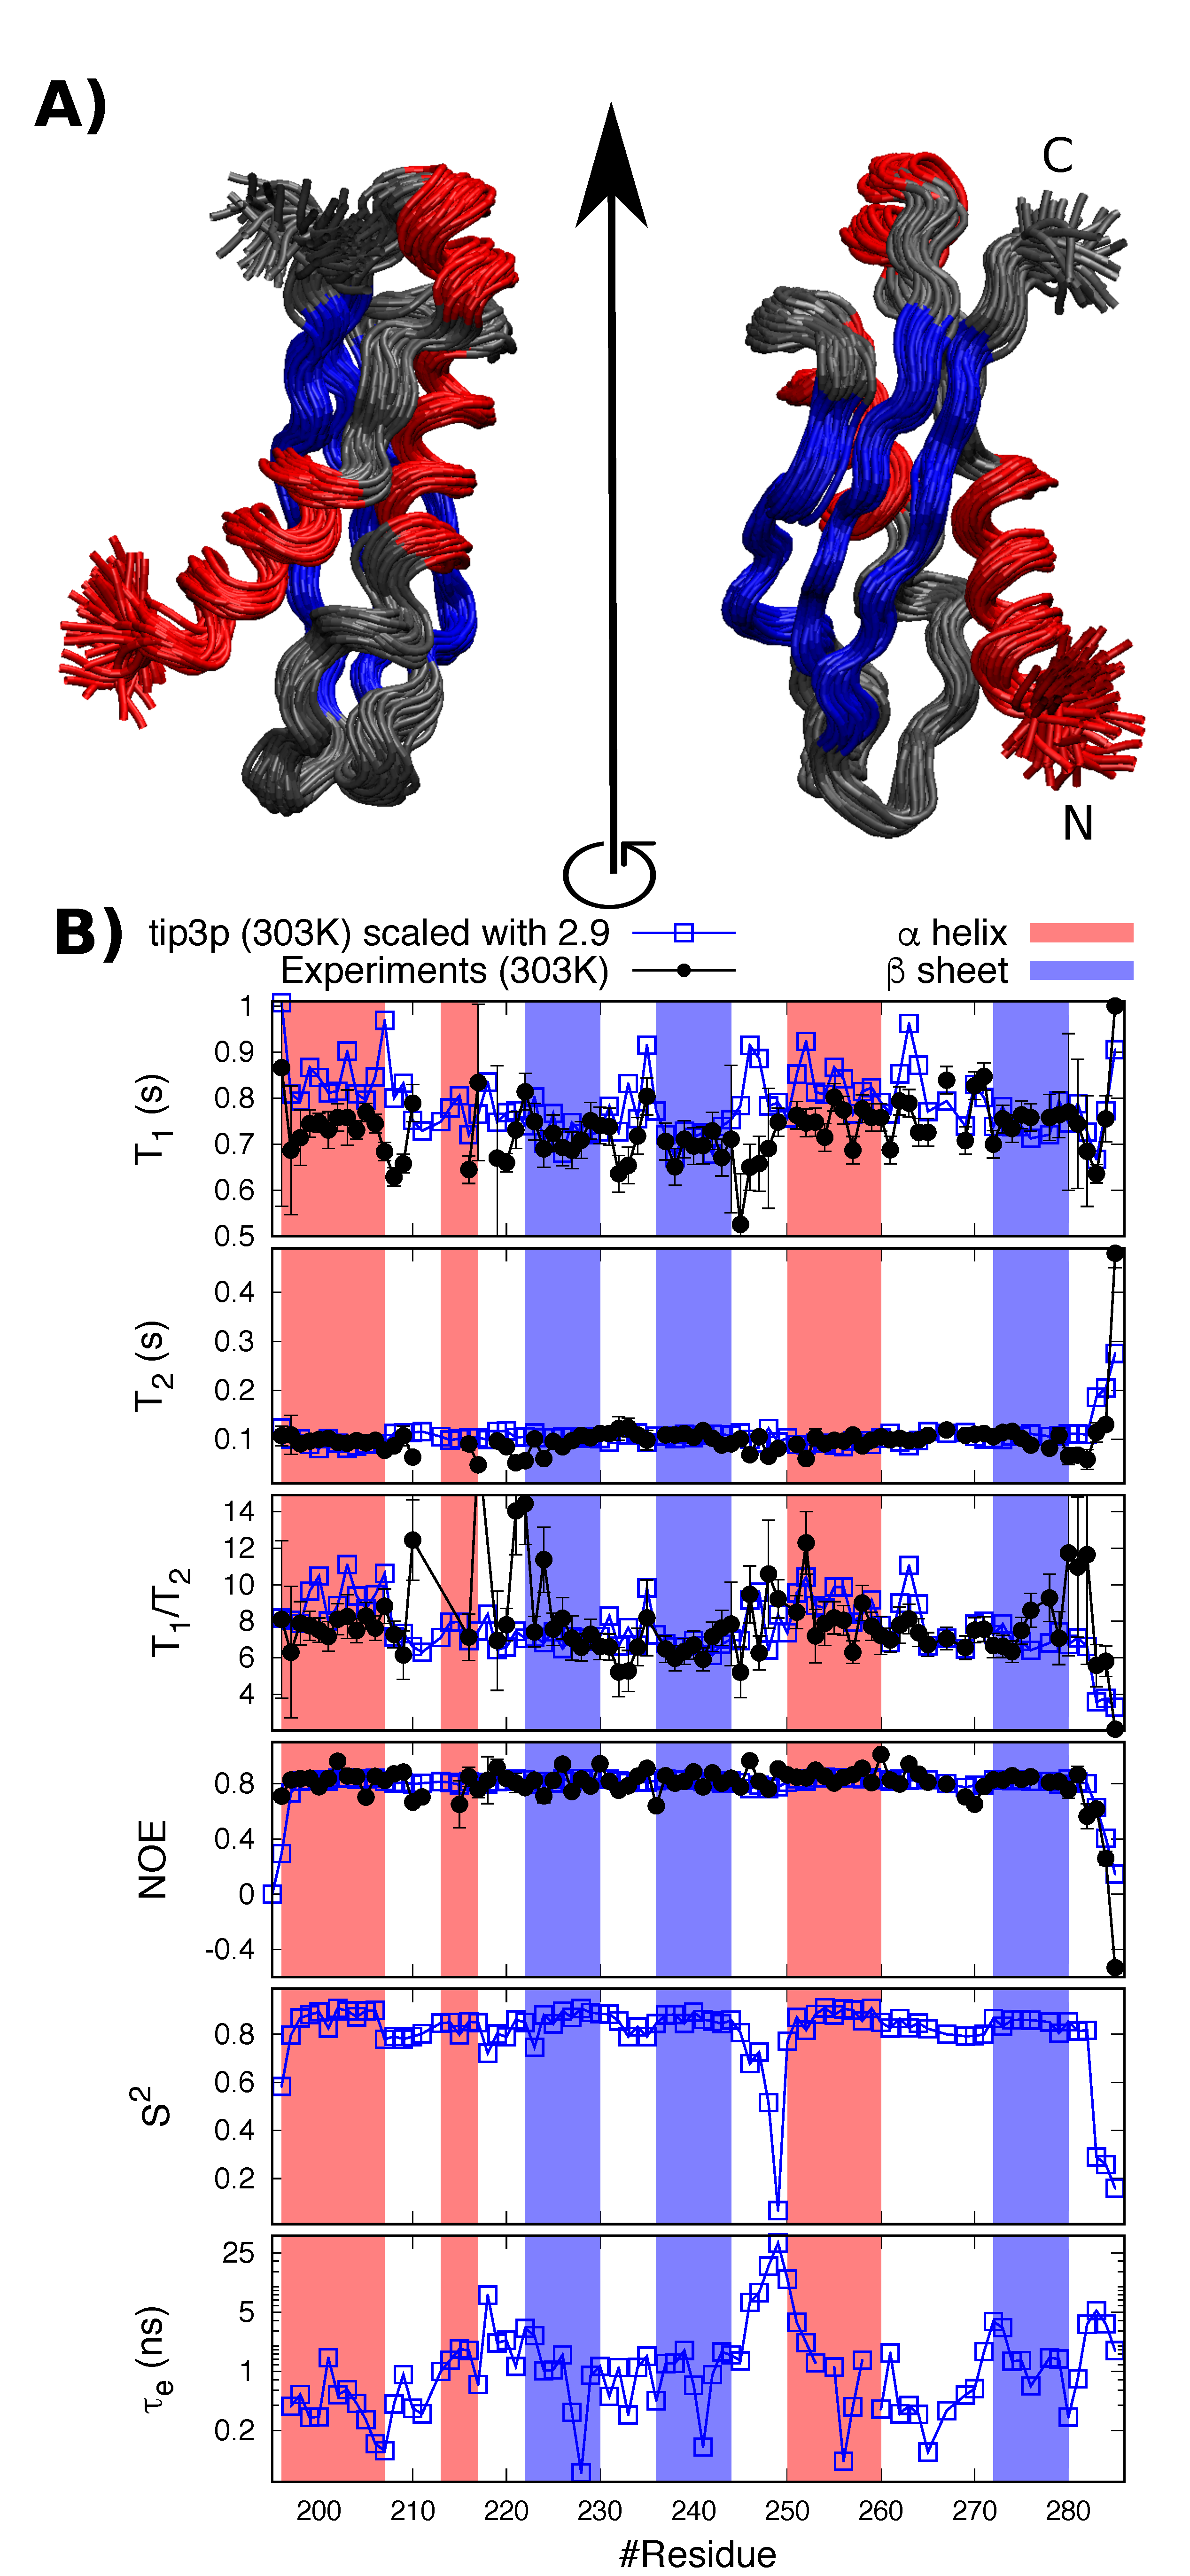
\includegraphics[width=8.0cm]{../Figs/RELdataHpTonB2.eps}%
  \caption{A) Structures of {\it Hp}TonB-92 from the MD simulations with tip3p at 303~K
    (100 structures taken from 400ns long trajectory). Secondary structures
    are color-labeled with Visual Molecular dynamics \cite{frishman95,humphrey96};
    $\alpha$-helices are red and $\beta$-strands are blue.
    Terminal ends are labelled with N and C.
    B) Spin relaxation times from experiments (circles) and tip3p
    simulations (squares) with rotational diffusion coefficients divided by a
    constant factor of 2.9 at 303~K. Order parameters and effective internal correlation
    times calculated from simulations
    \label{HpTonBrelaxationDATAscaled}}%
\end{figure}

Similar comparison for the spin relaxation times of {\it Pa}TonB-96 
between experiments and simulations with tip3p, tip4p and OPC4 water models
is shown in Fig. \ref{PsTonBrelaxationDATA}.
The experimentation of the OPC4 water model was inspired by the
recent study reporting significant improvements in lipid monolayer
simulations when this water model was used~\cite{javanainen18}. 
The underestimation of $T_1/T_2$ ratio was 
also observed in the simulations of {\it Pa}TonB-96 with
tip4p and OPC4 water models when compared with the experiments.
The discrepancy is, however, less severe than with tip3p, suggesting that 
the required scaling factor for the overall rotational diffusion should
be smaller for tip4p and OPC4 water models.
Indeed, the spin relaxation times calculated
from {\it Pa}TonB-96 simulation with tip4p water model
were found to be in good agreement with the experiments in Fig.~\ref{PsTonBrelaxationDATAscaled}
when the diffusion coefficients were divided with a constant factor of 1.2,
which is smaller than 2.9 used for the tip3p simulation of {\it Hp}TonB-92 above.
The scaling factors used to correct the overall rotational diffusion
of different proteins with different water models are shown in Table S1
together with the corresponding coefficients for self-diffusion of water \cite{wong08,izadi14}.
Notably, the effect of 12 degree temperature difference
on the spin relaxation times from tip4p simulations in Fig. \ref{PsTonBrelaxationDATA}
is significantly smaller than the observed differences between simulations and experiments or
the changes due to the scaling of the diffusion coefficient.
\begin{figure}[tb]
  \includegraphics[width=8.5cm]{../Figs/PsTonBrelaxationDATA.eps}%
  \caption{Plots of experimental (circles) and simulated (squares) spin relaxation times
    for {\it Pa}TonB-96. \label{PsTonBrelaxationDATA}}%
\end{figure}
\begin{figure}[p]
  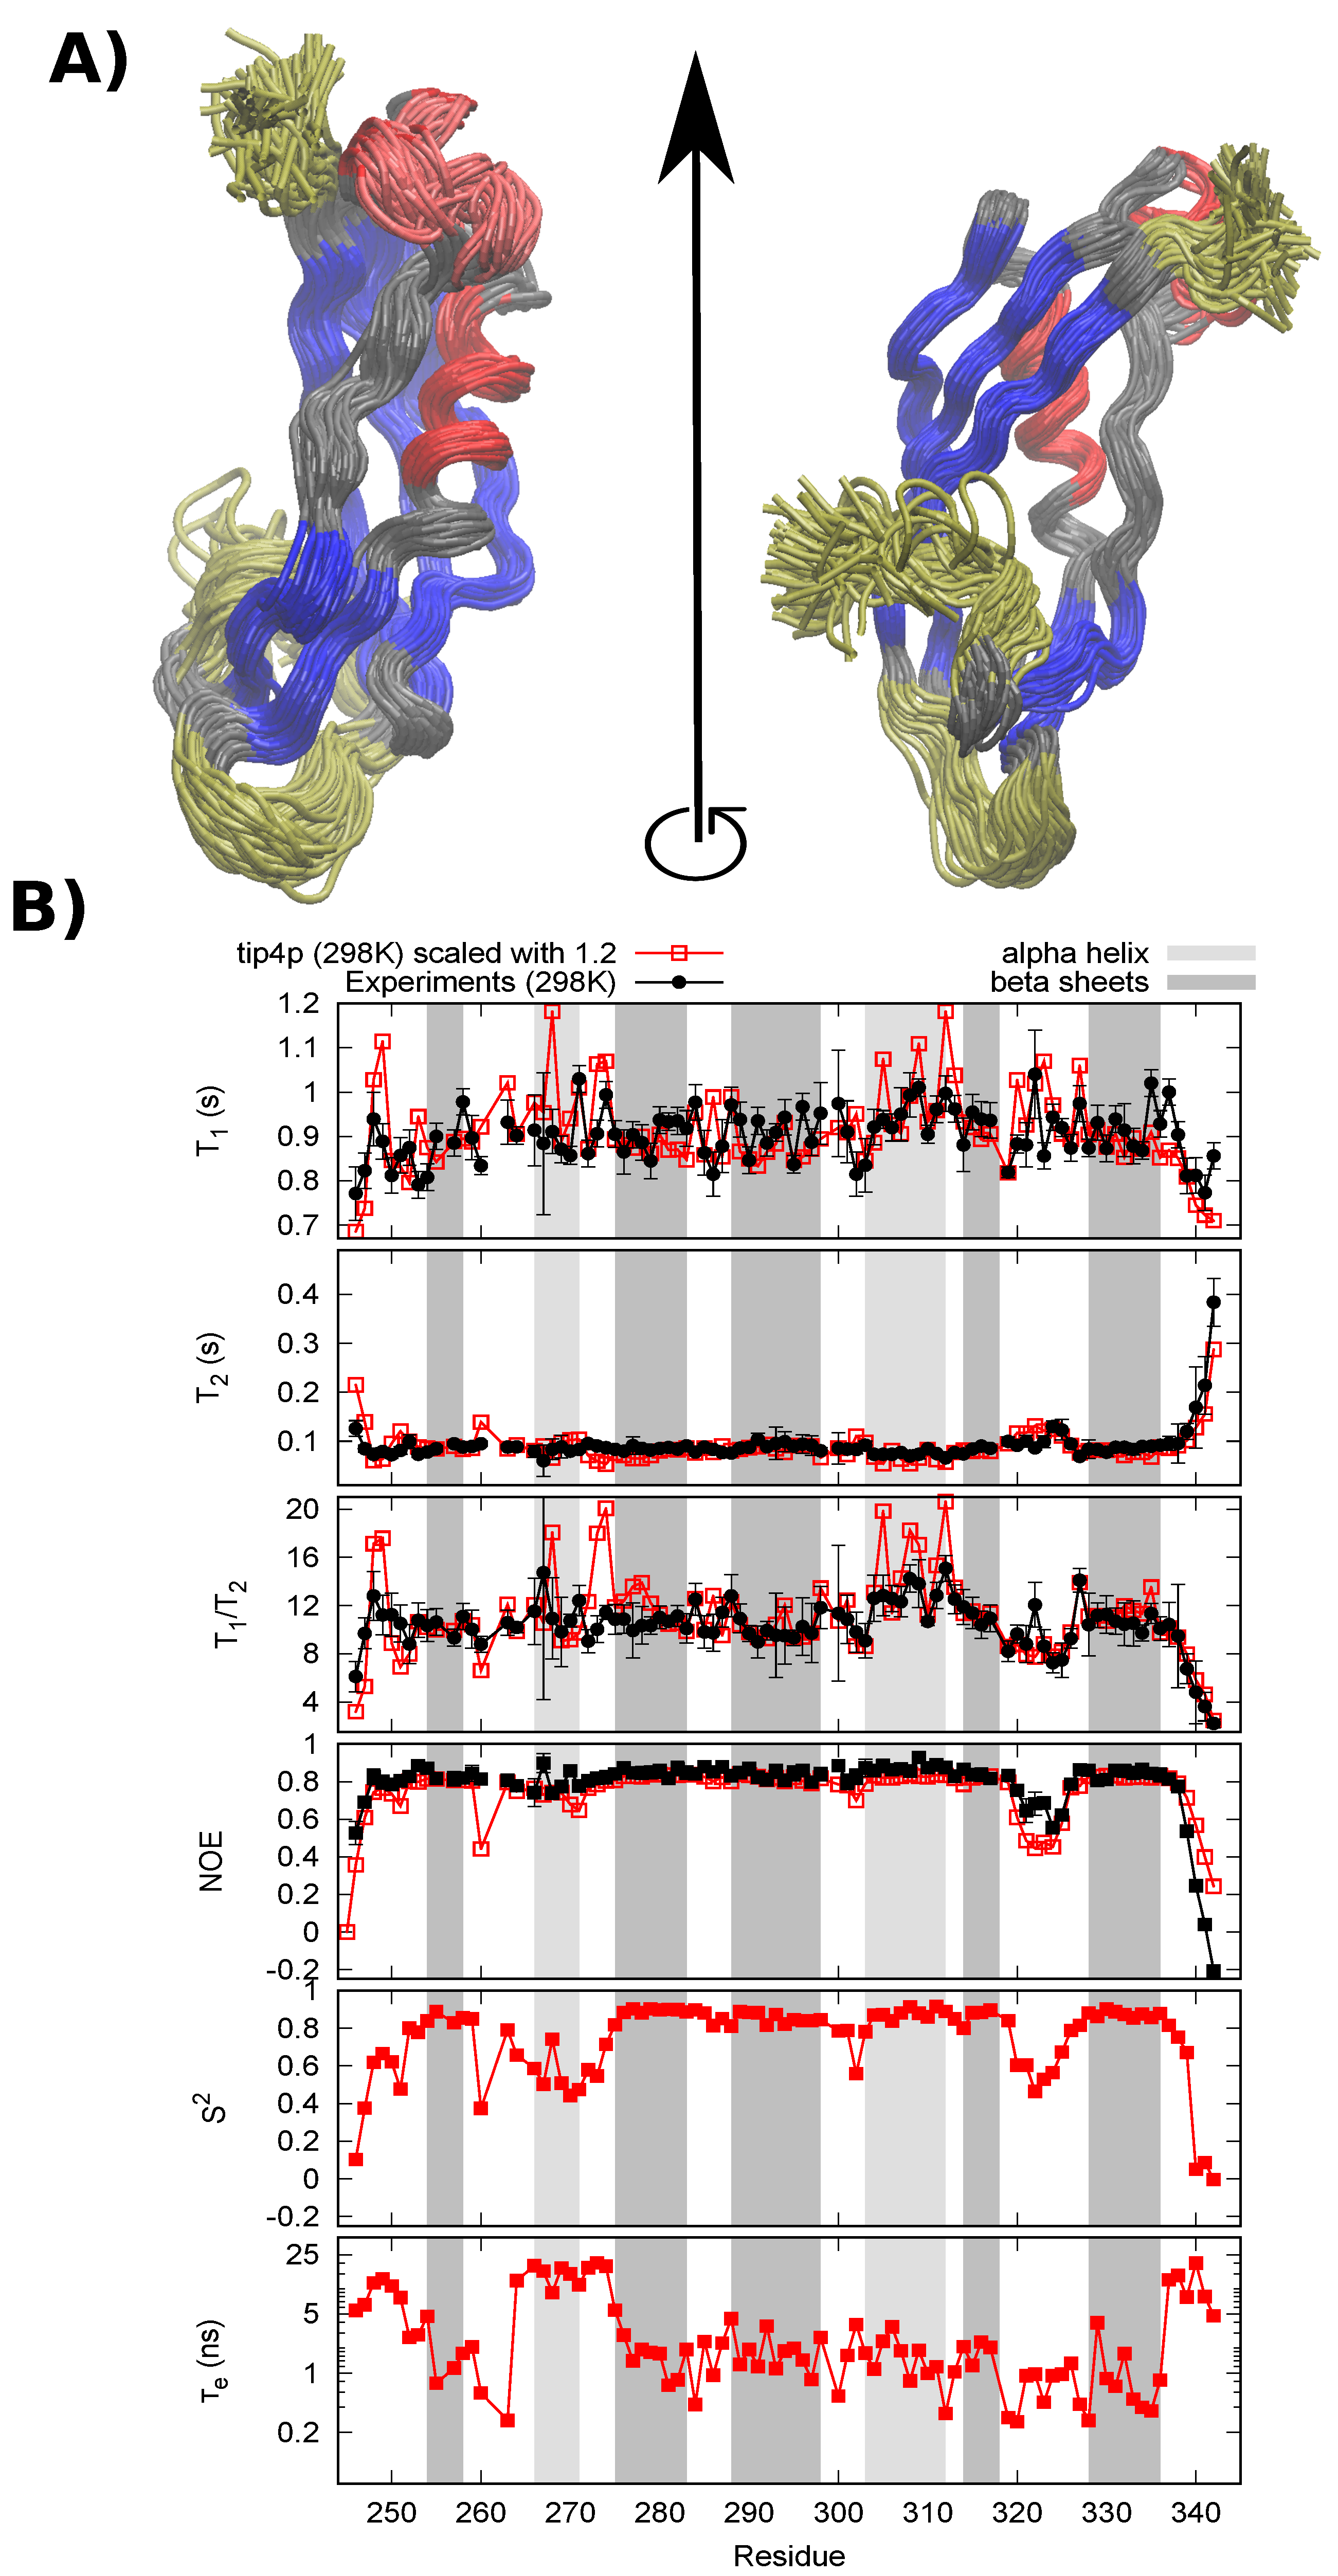
\includegraphics[width=8.0cm]{../Figs/RELdataPsTonB2.eps}%
  \caption{A) Structures sampled by {\it Pa}TonB-96 from MD simulations with tip4p at 298~K
    (100 structures from 400 ns long trajectory). Secondary structures
    are color labeled with Visual Molecular dynamics \cite{frishman95,humphrey96};
    $\alpha$-helixes and $\beta$-strands are red and blue, respectively.
    Residues 246-251, 320-326 and 338-342 with increased internal dynamics are yellow and
    $\alpha$-helix fluctuations between two orientations (residues 266-270) is violet in the left column.
    Terminal ends are labelled with N and C.
    B) Spin relaxation times from experiments (circles) and tip4p
    simulations (squares) with rotational diffusion coefficients divided by a
    constant factor of 1.2 at 298~K. Order parameters and effective internal correlation
    times calculated from simulations. \label{PsTonBrelaxationDATAscaled}}%
\end{figure}

The scaling of the overall rotational diffusion coefficients
with a constant factor led to a good agreement with the experimental
spin relaxation data for both systems simulated with different water models,
as seen in Figs.~\ref{HpTonBrelaxationDATAscaled} and~\ref{PsTonBrelaxationDATAscaled}.
The good agreement with experiments suggests that the scaled rotational diffusion coefficients
from MD simulations can be considered as a interpretation of the anisotropic rotational motion in NMR experiments.
The scaled rotational diffusion coefficients from the simulations giving the best agreement
with the experimental data are summarized in Table \ref{ROTdiffCOEFFSscaled}.
In contrast to the unscaled diffusion constants in Table~\ref{ROTdiffCOEFFS},
these results are in line with the previously reported values for proteins
with similar sizes~\cite{krishnan98}. Also the timescales, $\tau_{c}'$, estimated from 
Eq. \ref{ratioEQ} are close to the average diffusion coefficient, $\tau_{c}=(6D_{\rm av})^{-1}$,
in Table~\ref{ROTdiffCOEFFS}.
\begin{table}[!h]
  \centering
  \caption{Rotational diffusion coefficients (rad$^2\cdot 10^7$/s) giving the best agreement with experimental spin relaxation data.
    For {\it Hp}TonB-92 construct the values calculated from simulation with tip3p were scaled with 2.9
    (spin relaxation data in Fig.~\ref{HpTonBrelaxationDATAscaled}) and  for {\it Pa}TonB-96
    the values from tip4p simulation at 298K were scaled by 1.2 (spin relaxation data in
    Fig.~\ref{PsTonBrelaxationDATAscaled}). 
  }\label{ROTdiffCOEFFSscaled}
  \begin{tabular}{c c c c c}
    &    &  {\it Hp}TonB-92  &  & {\it Pa}TonB-96 \\
    \hline
    $D_{x}$        &    &   2.15 $\pm$ 0.01  & & 1.51  $\pm$ 0.01\\
    $D_{y}$        &    &  2.43  $\pm$ 0.01  & & 1.72  $\pm$ 0.03\\
    $D_{z}$        &    &  4.10   $\pm$ 0.01 & & 3.79  $\pm$ 0.03\\
    $D_{\rm av}$        &    &   2.90  $\pm$ 0.03  & & 2.3  $\pm$ 0.02\\
    $\tau_{c}$(ns)$^{\rm a}$  &    &  5.7   $\pm$ 0.1  & & 7.2 $\pm$ 0.1 \\
    $\tau_{c}'$(ns)$^{\rm b}$  &    &  5.8   $\pm$ 0.1 & & 6.9   $\pm$ 0.1 \\
    %\hline
  \end{tabular}
  \newline
  \flushleft
  $^{\rm a}\tau_{c}=(6D_{\rm av})^{-1}$, $^{\rm b}$Average over all residues given by Eq. \ref{ratioEQ}.
\end{table} 


\subsection{Interpretation of protein internal relaxation from MD simulations}
The good agreement of the spin relaxation times between the simulations
with the scaled overall rotational diffusion coefficients and
the experiments (Figs. \ref{HpTonBrelaxationDATAscaled} and \ref{PsTonBrelaxationDATAscaled})
suggest that the simulations can be used to interpret the internal
mobility of proteins from the experimental data.

Only small variations between different residues are observed
for spin relaxation times of {\it Hp}TonB-92 in Fig. \ref{HpTonBrelaxationDATAscaled}.
This indicates a rather rigid protein structure, which is also seen in
the MD simulation snapshots overlayed in Fig. \ref{HpTonBrelaxationDATAscaled} A).
Only few residues in the terminal ends show slightly
enhanced conformational fluctuations in the MD simulation and in
spin relaxation data. In addition, some deviations from the average spin relaxation times
are observed in the experimental data close to residues 210-222.
Simulations of {\it Hp}TonB-92 do not offer any explanation for this
observation, however, the similar region in {\it Pa}TonB-96 simulation shows 
fluctuations between two orientations of $\alpha$-helix \cite{oeemig17}.
Exceptionally low order parameters and long effective correlation times 
are observed in simulations for residues 245-250 of {\it Hp}TonB-92.
Moreover, short $T_1$ times are experimentally observed close to this region,
but the interpretation is not straightforward as the low $T_1$ times
are not reproduced by MD simulations.

{\it Pa}TonB-96 exhibits more internal mobility 
and the segments with enhanced conformational fluctuations are labeled with yellow color
in Fig. \ref{PsTonBrelaxationDATAscaled}.
Larger number of sampled conformations in both terminal ends
are characterized by low order parameters and long effective internal correlation times
observed in the simulations. 
Enhanced conformational fluctuations are also observed for residues 320-326,
which correspond the loop between two $\beta$-strands.
MD simulations predict low order parameters and long internal effective correlation
times also close to residues 266-271, which can be explained by  
two different orientations sampled by the $\alpha$-helix in this region
(color labeled with violet in Fig.~\ref{PsTonBrelaxationDATAscaled} A).
The orientational fluctuations of the similar short helix could also explain the above mentioned
deviations of spin relaxation times for residues 210-222 of {\it Hp}TonB-92~\cite{ciragan16}.

MD simulations can be used to analyze different components contributing to
the rotational dynamics of individual N-H bonds.
In this work we have fitted a sum of 471 different
timescales to the correlation functions according to Eq.~\ref{gprime_fit}.
Most of the prefactors ($\alpha_i$ in Eq.~\ref{gprime_fit}) are zero
in all the correlation functions after the fitting,
thus the timescales $\tau_i$ corresponding non-zero prefactors
are considered as the components contributing to the total relaxation process of each N-H bond.
The prefactors are shown in Fig. \ref{coeffsPLOT} for the same residues
of {\it Pa}TonB-96, which were used to exemplify the correlation functions in Fig. \ref{exampleCORRF}.
As expected for residue 322 in the rigid $\beta$-sheet with large order parameter,
the rotational relaxation is dominated by timescales of $\sim$5.5~ns and $\sim$8~ns,
matching with the protein overall
rotation. Also the dynamics of residue 322 in the flexible loop of {\it Pa}TonB is
dominated by the timescales around $\sim$8~ns corresponding to the protein overall rotation,
however, the fast motions from internal mobility are more evident than for the
rigid $\beta$-sheet residue. This is in agreement with smaller order parameter observed
in the flexible loop residues. On the other hand, the rotational dynamics of
residue 341 in the flexible N-terminus of {\it Pa}TonB is dominated by timescales
below 3~ns, most likely related to the internal motion of the protein.
Contributions from timescales around $\sim$13~ns to the dynamics of residue 341 probably
arise from the slow conformational fluctuations of the N-terminus, rather than the overall
rotational dynamics. This supports the conclusion that the large amount of sampled
conformations lead to the small order parameters and large effective correlation times
observed in Fig. \ref{PsTonBrelaxationDATA}.
While the separation of rotational dynamics of individual N-H bonds to different components
gives intuitively understandable results, it should be kept in mind that
it is based on the fitting of a multiexponential sum to the simulation data and the solution
of such fit is not unique.
\begin{figure}[!h]
  \includegraphics[width=8.5cm]{../Figs/coeffsPLOT.eps}%
  \caption{Prefactors $\alpha_i$ corresponding different timescales $\tau_i$
    resulting from a fit of Eq.\ref{gprime_fit} to correlation functions from
    MD simulation of {\it Pa}TonB-96 at 298K. The used correlation functions give
    a good agreement with experimental spin relaxation times as shown in
    Fig.~\ref{PsTonBrelaxationDATAscaled}.  \label{coeffsPLOT}}%
\end{figure}


\section{Conclusions}
The experimental spin relaxation data for protein backbone N-H bonds
was successfully reproduced by using the classical molecular dynamics
simulations for two different small domains.
Thus, the simulation trajectories give an atomic resolution
interpretation for protein dynamics measured with NMR experiments.
Interpretation of the overall and internal dynamics was demonstrated for
two proteins with anisotropic molecular shape and some flexible regions. 
Interpretation of the $^{15}$N spin relaxation data measured from
such proteins has been very challenging with the previously available
methods~\cite{barbato92,luginbuhl97}.

The overall rotation of the studied proteins was found to be Brownian having
only a small subdiffusive behavior with short timescales
below~$\sim$0.12 ns, which could be contrasted with crowded environments,
where anomalous diffusion is expected to be more significant \cite{hofling13}.
The direct analysis of classical molecular dynamics trajectories did not, however,
reproduce the experimental $^{15}$N spin relaxation data. Comparison between the rotational 
diffusion coefficients and spin relaxation times between simulations
and experiments suggested that
the overall Brownian tumbling of proteins is too rapid in the simulations,
in agreement with the previous report suggesting that the discrepancy arises
from the inaccuracies in water models~\cite{wong08,takemura12,debiec16}.
Scaling down the anisotropic diffusion coefficients in the simulation data
led to a good agreement with the experimental data.
Overall rotational diffusion coefficients were overestimated by a factor of $\sim$3 in
the {\it Hp}TonB-92 simulations with tip3p water model, in line with previous
studies \cite{prompers02,wong08,anderson12,linke18}. Simulations with tip4p and OPC4
water models gave the spin relaxation times in reasonable agreement with experiments
with scaling factors of $\sim$1-1.2, which is significantly less than for tip3p.
%It should be noted, however, that the correct scaling factors for 
%the two different proteins, {\it Hp}TonB-92 and {\it Pa}TonB-96, simulated with the
%same water model, tip4p, seems to be 1 and 1.2, respectively. This suggests
%that the correction factor is not fully determined by the bulk water properties
%and that the hydration layer and water-protein interactions may play a critical
%role in rotational dynamics of proteins, as also suggested by the hydrodynamical 
%calculations \cite{torre00}.
The scaling factors for different proteins with
different water models are summarized in Table S1.

Similarity between the correlation functions from the original MD trajectory and
the new correlation functions from Eq.~\ref{newCORRF} 
suggest that the usage of the inertia axes
and the separation of internal and the overall rotational motions
(Eq.~\ref{CORRFsep}) are good approximations for the above investigated
proteins. This is in line with the previous studies of other  
proteins with well defined structure~\cite{wong08,allner15}. However, it remains to be seen
how well this and other related approaches~\cite{prompers02,anderson12,chia18} 
will succeed for intrinsically disordered proteins without
the well defined shape. Since the correction of the incorrect overall
rotational diffusion due to water model may become highly complicated for such proteins,
it may be necessary to employ a water model giving correct
overall rotational diffusion coefficients for biomolecules \cite{takemura12,debiec16}.

As further demonstrated in Ref.~\citenum{oeemig17}, the approach presented in this work can be used to interpret the
rotational dynamics of proteins with anisotropic shape from $^{15}$N
spin relaxation data measured only with one magnetic field strength.
This is a significant advancement over currently available methods,
which may not be applicable in such cases, even thought experimental
data would be measured with multiple magnetic field strengths.


%%%%%%%%%%%%%%%%%%%%%%%%%%%%%%%%%%%%%%%%%%%%%%%%%%%%%%%%%%%%%%%%%%%%%
%% The "Acknowledgement" section can be given in all manuscript
%% classes.  This should be given within the "acknowledgement"
%% environment, which will make the correct section or running title.
%%%%%%%%%%%%%%%%%%%%%%%%%%%%%%%%%%%%%%%%%%%%%%%%%%%%%%%%%%%%%%%%%%%%%
\begin{acknowledgement}
  Academy of Finland (277335) and Sigrid Jus{\' e}lius Foundation are acknowledged for the financial support
  to complete this work. The Finnish Biological NMR Center is supported by Biocenter Finland and HiLIFE-INFRA.
  We acknowledge CSC-IT center for science for computational resources.
\end{acknowledgement}

%%%%%%%%%%%%%%%%%%%%%%%%%%%%%%%%%%%%%%%%%%%%%%%%%%%%%%%%%%%%%%%%%%%%%
%% The same is true for Supporting Information, which should use the
%% suppinfo environment.
%%%%%%%%%%%%%%%%%%%%%%%%%%%%%%%%%%%%%%%%%%%%%%%%%%%%%%%%%%%%%%%%%%%%%
\begin{suppinfo}

%A listing of the contents of each file supplied as Supporting Information
%should be included. For instructions on what should be included in the
%Supporting Information as well as how to prepare this material for
%publications, refer to the journal's Instructions for Authors.

%The following files are available free of charge.
  \begin{itemize}
  \item Mean square angle deviations of {\it Pa}TonB-96 simulations with tip4p water at 310~K and 298~K
  \item Accuracy estimation of the scaling factors for the rotational diffusion
\end{itemize}

\end{suppinfo}

%%%%%%%%%%%%%%%%%%%%%%%%%%%%%%%%%%%%%%%%%%%%%%%%%%%%%%%%%%%%%%%%%%%%%
%% The appropriate \bibliography command should be placed here.
%% Notice that the class file automatically sets \bibliographystyle
%% and also names the section correctly.
%%%%%%%%%%%%%%%%%%%%%%%%%%%%%%%%%%%%%%%%%%%%%%%%%%%%%%%%%%%%%%%%%%%%%
\bibliography{refs}

\end{document}
